\documentclass[12pt,letterpaper]{article}
\usepackage[utf8]{inputenc}
\usepackage{amsmath,amsthm,amsfonts,amssymb,amscd}
\usepackage[table]{xcolor}
\usepackage[margin=2.5cm]{geometry}
\usepackage{ragged2e}
\usepackage{graphicx}
\usepackage{multicol}
\newlength{\tabcont}
\setlength{\parindent}{0.0in}
\setlength{\parskip}{0.05in}

\begin{document}
	
	\large \textbf{Nome}: Luís Felipe de Melo Costa Silva \\
	\textbf{Número USP}: 9297961 
    
	\begin{center}
		\LARGE \bf
		Lista de Exercícios 3 - MAC0444
	\end{center}

	\begin{normalsize}
		\section*{Exercício 1}
		
		\textbf{a)} O conceito descreve um ser humano que não é do sexo feminino, que existe um médico que é casado com ele, e que todos os seus filhos são professores ou médicos.
		
		\textbf{b)} Usando uma interpretação de mundo fechado, nenhuma das quatro pessoas mencionadas pertencem a esse conceito. Interpretando o mundo como aberto, não há como ter certeza disso, pois Marta pode ser médica ou professora, embora esteja desempregada.
		
		\textbf{c)} Sim, se Marta não existisse, a resposta com uma interpretação de mundo fechado seria de que Pedro pertence a esse conceito.
		
		\section*{Exercício 2}
		
		\section*{Exercício 3}
		
		Vamos traduzir a sentença: \\
		
		$PaiDeMedicos \sqsubseteq \exists temFilho(Homem \sqcup Mulher) \sqcap \forall temFilho(Medico)$
		
		$\forall x(t_x(PaiDeMedicos)) \to t_x(\exists temFilho(Homem \sqcup Mulher) \sqcap \forall temFilho(Medico)))$
		
		$\forall x(PaiDeMedicos(x) \to t_x(\exists temFilho(Homem \sqcup Mulher) \sqcap \forall temFilho(Medico)))$
		
		$\forall x(PaiDeMedicos(x) \to t_x(\exists temFilho(Homem \sqcup Mulher)) \land t_x(\forall temFilho(Medico)))$
		
		$\forall x(PaiDeMedicos(x) \to \exists y(temFilho(x,y) \land t_y(Homem \sqcup Mulher)) \land t_x(\forall temFilho(Medico)))$
		
		$\forall x(PaiDeMedicos(x) \to \exists y(temFilho(x,y) \land (t_y(Homem) \lor t_y(Mulher))) \land t_x(\forall temFilho(Medico)))$
		
		$\forall x(PaiDeMedicos(x) \to \exists y(temFilho(x,y) \land (Homem(y) \lor Mulher(y))) \land t_x(\forall temFilho(Medico)))$
		
		$\forall x(PaiDeMedicos(x) \to \exists y(temFilho(x,y) \land (Homem(y) \lor Mulher(y))) \land t_x(\forall temFilho(Medico)))$
		
		$\forall x(PaiDeMedicos(x) \to \exists y(temFilho(x,y) \land (Homem(y) \lor Mulher(y))) \land \forall y(temFilho(x,y) \to t_y(Medico)))$
		
		$\forall x(PaiDeMedicos(x) \to \exists y(temFilho(x,y) \land (Homem(y) \lor Mulher(y))) \land \forall y(temFilho(x,y) \to Medico (y))$
		
		\section*{Exercício 4}
		
		Para provarmos que $Vegano \sqsubseteq Vegetariano$, temos que mostrar que $Vegano$ $\sqcap$ $\lnot Vegetariano$ é insatisfazível.
		
		$\lnot Vegetariano = (\lnot Homem \sqcap \lnot Mulher) \sqcup \exists come(\lnot Planta \sqcap \lnot Laticinio)$
		
		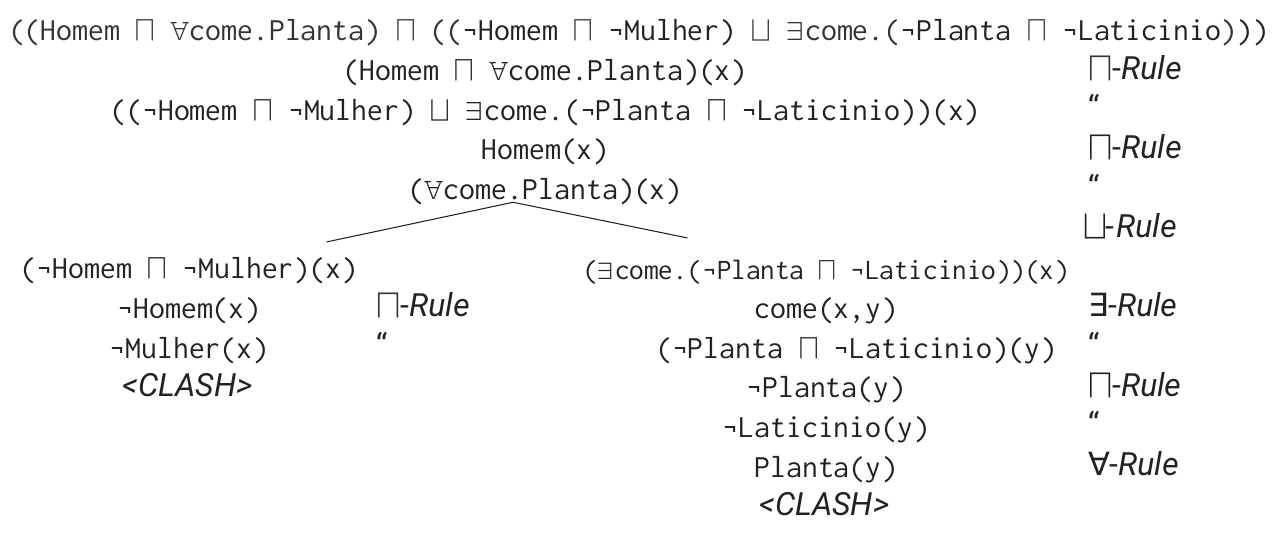
\includegraphics[width=17cm]{ex4.png}
		
		Portanto, $Vegano \sqsubseteq Vegetariano$.
	\end{normalsize}
			 
\end{document}